%!TEX root =  free234.tex
\null \vfill

\noindent
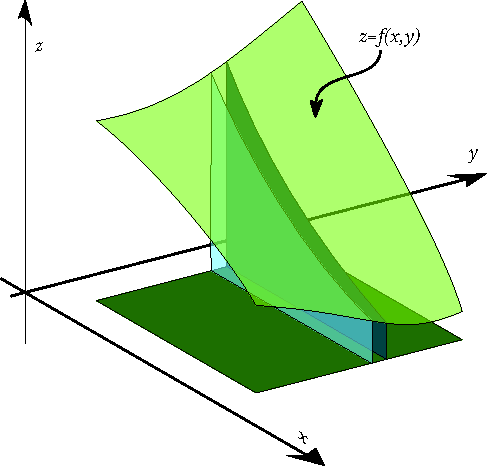
\includegraphics[width=0.7\textwidth]{04slice1.pdf}

\begin{flushright} \huge\sffamily\bfseries%
  MATH 234 \\
  THIRD SEMESTER \\
  CALCULUS\\[1in]
  \large \semester
\end{flushright}

\vfill \newpage
\vfill

\begin{center}
  \bfseries Math 234 -- 3rd Semester Calculus \\
  Lecture notes version \version (\semester)
\end{center}

\noindent This is a self contained set of lecture notes for Math 234. The
notes were written by Sigurd Angenent, some problems were
taken from Guichard's open calculus text which is available at
\url{http://www.whitman.edu/mathematics/multivariable/src/}

The \LaTeX\ files, as well as the \textsc{Python} and \textsc{Inkscape-svg}
files that were used to produce the notes before you can be obtained from
the following web site:
\begin{center}
  \url{http://www.math.wisc.edu/~angenent/Free-Lecture-Notes}
\end{center}
They are meant to be freely available for non-commercial use, in the sense
that ``free software'' is free. More precisely:

\bigskip

\begin{center}
  \framebox{
  \begin{minipage}[b]{4.5in}\raggedright\footnotesize
    Copyright (c) 2009 Sigurd B. Angenent. Permission is granted
    to copy, distribute and/or modify this document under the
    terms of the GNU Free Documentation License, Version 1.2 or
    any later version published by the Free Software Foundation;
    with no Invariant Sections, no Front-Cover Texts, and no
    Back-Cover Texts.  A copy of the license is included in the
    section entitled "GNU Free Documentation License".
  \end{minipage}
  }
\end{center}
\vfill
%\begin{flushright}
%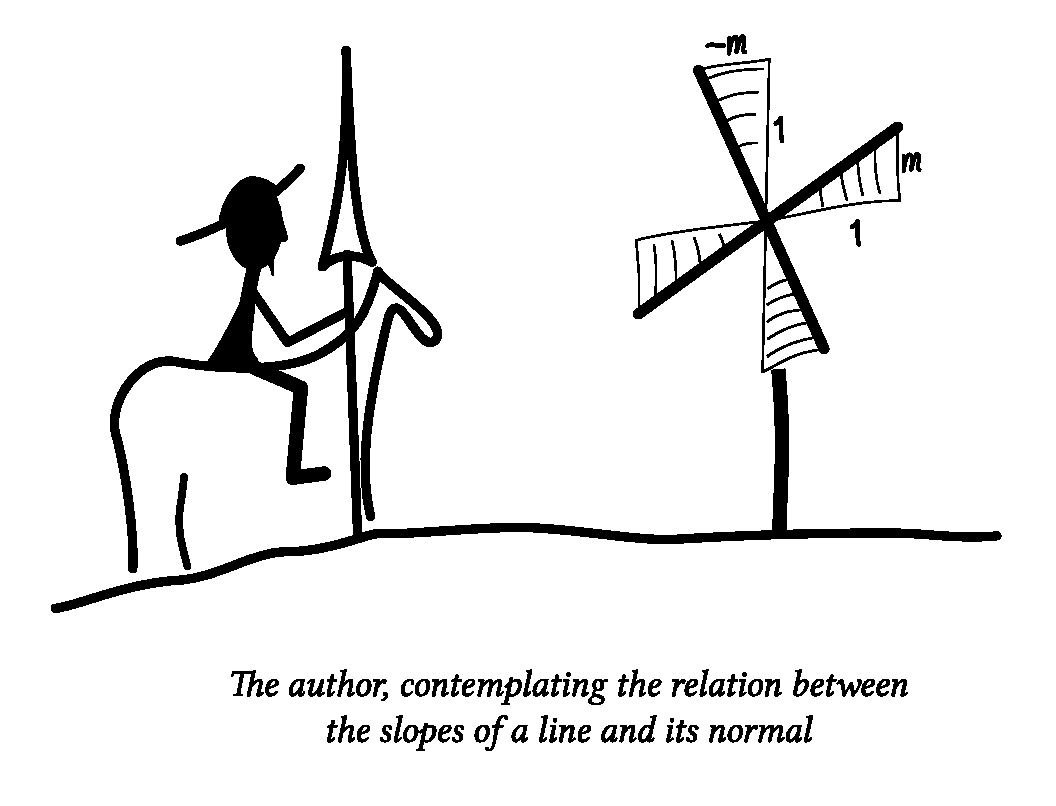
\includegraphics[width=0.7\textwidth]{donQ.pdf}
%\end{flushright}
\newpage

%\begin{multicols}{2}
\begingroup
\footnotesize\sffamily
\tableofcontents
\endgroup
%\end{multicols}

%\setlength{\parskip}{3pt plus 3pt}
%\section*{From the department's syllabus}
%\problem
%Which topics are supposed to be covered in this course at UW Madison?
%\answer The topics are
%
%-- Vector functions and space curves, velocity and acceleration
%
%-- Arc length and curvature, normal and binormal
%
%-- Motion in space, planetary motion
%
%-- Partial derivatives
%
%-- Tangent planes and normals
%
%-- Linear approximation
%
%-- gradient and total differential
%
%-- Local and absolute extrema
%
%-- Lagrange multipliers
%
%-- Higher derivatives, exact differentials
%
%-- Double and iterated integrals, including polar coordinates
%
%-- Applications of double integrals
%
%-- Triple and iterated integrals, including cylindrical and
%  spherical coordinates
%
%-- Applications of triple integrals, volume and surface areas.
%
%-- Vector fields, surface integrals and line integrals
%
%-- Flux, Green's theorem
%
%-- Divergence Theorem, Stokes' theorem
%
%\endanswer
%
